\section{Digital Link}
\subsection{Lecture 18}

\subsubsection{MAP/MLE}

We now turn to the problem of transfering information reliably (i.e. meeting performance requirements) using
minimum resources (computation, bandwidth, storage, energy, ...). This is across a physical
medium: which could be a phone line cable, fiber or wireless.

To do this, we often have to formulate multiple types of estimation problems. First, we talk about Bayes' Rule.
Let $C_1, \dots, C_N$ are "circumstances," while $S$ is a certain "symptom." Observing a particular symptom $S$,
what circumstance happened?

We are given "priors" $p_i = \Pr{C_i}$ (how frequent in the population that circumstance $C_i$ is)
and "conditionals" $q_i = \Pr{S \mid C_i}$ (how likely you are to have symptom $S$ if you have circumstance $C_i$).

\begin{theorem}[Bayes' Rule]
    Define $\pi_i = \Pr{C_i \mid S}$. Then $\pi_i = \frac{p_i q_i}{\sum_{j = 1}^N p_j q_j}$.
    Note that the bottom probability is just the probability of the symptom, $\Pr{S}$.
\end{theorem}

This leads to two ways to estimate what a circumstance you have.

\begin{definition}[MAP/MLE for events]
    The Maximum A Posteriori estimate (MAP) is defined as:
    \[ MAP = \argmax_i \Pr{C_i \mid S} = \argmax_i p_i q_i \]
    and the Maximum Likelihood Estimate (MLE) is defined as:
    \[ MLE = \argmax_i \Pr{S \mid C_i} = \argmax_i q_i \]
\end{definition}

Note that if all the priors are the same, then the MAP and MLE are the same.
We can also extend this to general discrete random variables:
\begin{definition}[MAP/MLE for Discrete RVs]
    Let $X$ and $Y$ be discrete random variables.
    \[ MAP[X \mid Y = y] = \argmax_x \Pr{X=x, Y=y} \]
    \[ MLE[X \mid Y = y] = \argmax_x \Pr{Y = y \mid X = x} \]
\end{definition}

We think of $Y$ as an output we "observe"; we want to know what input $X$ caused this.

First, we take the case of a Binary Symmetric Channel (BSC).

\[\begin{tikzcd}
	X & 0 && 0 & Y \\
	& 1 && 1
	\arrow["{1-p}", from=1-2, to=1-4]
	\arrow["p"'{pos=0.3}, from=2-2, to=1-4]
	\arrow["p"{pos=0.3}, from=1-2, to=2-4]
	\arrow["{1-p}"', from=2-2, to=2-4]
\end{tikzcd}\]

We transmit either a 0 or 1 from an input $X$
and get a 0 or 1 in the output $Y$ and the channel has a probability $p$ of corrupting the packet.
Furthermore, let $\Pr{X = 1} = \alpha$ (the prior). Then,

\begin{theorem}
    For the BSC,
    \[ MAP[X \mid Y = y] = \begin{cases}
        \mathbbm{1}\{\alpha > (1 - p)\} & y = 0 \\
        \mathbbm{1}\{\alpha > p\} & y = 1 \\
    \end{cases} \]
    and
    \[ MLE[X \mid Y] = \begin{cases}
        Y & p < 0.5 \\
        |Y - 1| & p \geq 0.5
    \end{cases} \]
    where the last expression just flips the observation $Y$.

    We can derive this with a straightforward Bayes Rule calculation using the previous facts. I'll omit the calculations.
\end{theorem}

Now, we discuss the additive Gaussian Noise channel, $Y = X + Z$ where $\Normal{Z}{0}{\sigma^2}$ is independent of $X$.
Suppose $X \in \{0, 1\}$. Let $f_0 = f_{Y \mid X = 0}$ and $f_1 = f_{Y \mid X = 1}$. Furthermore, call the priors $p_0, p_1$.

Let $\epsilon << 1$, then
\begin{align*}
    q_0 &= \Pr{Y \in (y, y + \epsilon] \mid X = 0} \\
    &= f_0(y) \epsilon \\
    q_1 &= \Pr{Y \in (y, y + \epsilon] \mid X = 1} \\
    &= f_1(y) \epsilon \\
\end{align*}
Thus, we can just compare densities.
\begin{align*}
    MAP[X \mid Y = y] = \argmax_{i \in \{0, 1\}} p_i f_i(y) \\
    p_1 \frac{e^{\frac{-{y - 1}^2}{2 \sigma^2}}}{\sqrt{2\pi} \sigma} > p_0 \frac{e^{\frac{-y^2}{2 \sigma^2}}}{\sqrt{2\pi} \sigma} \\
\end{align*}
this will simplify algebraically to our result below. The MLE is just comparing $q_0$ and $q_1$:
\begin{align*}
    MLE[X \mid Y = y] &= \argmax_{i \in \{0, 1\}} f_i(y) \\
\end{align*}
However, by symmetry, the two normal curves intersect at $y = \frac{1}{2}$, so the $q_1$ over takes $q_0$ if $y \geq \frac12$.

\begin{theorem}
    For the Gaussian channel,
    \[ MAP[X \mid Y = y] = 1\{ y \geq \frac12 + \sigma^2 \ln\qty(\frac{p_0}{p_1})\}\]
    \[ MLE[X \mid Y = y] = 1\{ y \geq \frac12 \}\]
\end{theorem}

In turn, we can calculate the probability of error under MLE. That is, we transmitted a 0 but got $y \geq \frac12$ and misclassified it
as a 1. Call the probability $p$
\begin{align*}
    p &= p_0 \Pr{Z \geq 0.5} + p_1 \Pr{Z + 1 < 0.5} \\
    p &= p_0 \Pr{Z \geq 0.5} + p_1 \Pr{Z < -0.5} \\
    p &= p_0 \Pr{Z \geq 0.5} + p_1 \Pr{Z \geq 0.5} \\
    p &= \Pr{Z \geq 0.5} \\
\end{align*}

\subsubsection{Huffman Codes}

Consider the problem of coding 4 symbols $A, B, C, D$ in a piece of text into binary. One option is assign:
\[ A = 00, B = 01, C = 10, D = 11 \]
We can decode a received string without errors unambiguously. We have to use two bits per symbol.

Now, suppose we have additional information: the frequency of occurrence of each symbol is
0.55, 0.3, 0.1, 0.05 respectively. Let's assign 0, 10, 110, 111 to $A, B, C, D$ respectively.
The reason we are doing this is because we are assigning shorter codes to more frequent symbols.
Here, we can also unambiguously decode in one pass since the codes are prefix-free (no code is a prefix of
any other). If we compute the average number of bits per symbol, this is now 1.6 (saving us a lot of bits).

This is how we constructed the code. The code is prefix tree because all codewords lie at a leaf node (none is an ancestor of another).

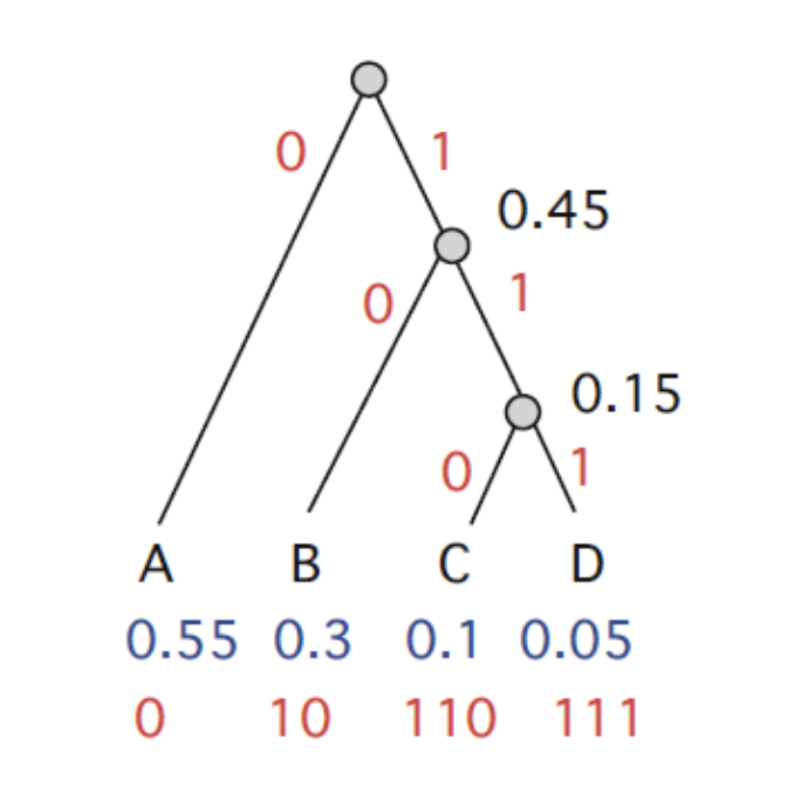
\includegraphics[width=50mm]{huffmantree.png}

The way we found the codewords is through the following algorithm.

\begin{note}[Huffman Coding Algorithm]
    We are given a list of symbols $i$ with probabilities $p_i$. The Huffman tree is built as follows:
    \begin{itemize}
        \item Take the two symbols with smallest probability $a$ and $b$.
        \item Put them as leaves on a tree and combine them into a root $\{a, b\}$ with probability $p_a + p_b$.
        \item Iteratively continue this, considering $\{a, b\}$ as one character with its new probability (and $a, b$ removed).
    \end{itemize}
\end{note}

\begin{theorem}
    The Huffman Code has the smallest average number of bits per symbol among all prefix-free codes.
\end{theorem}

We will see next lecture why this is the case.